% Sandia National Laboratories is a multimission laboratory managed and
% operated by National Technology & Engineering Solutions of Sandia, LLC, a
% wholly owned subsidiary of Honeywell International Inc., for the U.S.
% Department of Energy’s National Nuclear Security Administration under
% contract DE-NA0003525.

% Copyright 2002-2020 National Technology & Engineering Solutions of Sandia,
% LLC (NTESS).


\begin{Device}\label{L_DEVICE}

\symbol
{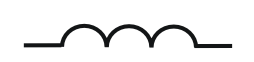
\includegraphics{inductorSymbol}}

\device
L<name> <(+) node> <(-) node> [model] <value> [device parameters]

\model
\begin{alltt}
.MODEL <model name> L [model parameters]
.MODEL <model name> IND [model parameters]
\end{alltt}

\examples
\begin{alltt}
L1 1 5 3.718e-08
LM 7 8 L=5e-3 M=2
LLOAD 3 6 4.540mH IC=2mA
Lmodded 3 6 indmod 4.540mH
.model indmod L (L=.5 TC1=0.010 TC2=0.0094)
\end{alltt}

\parameters

\begin{Parameters}
\param{\vbox{\hbox{(+) node\hfil}\hbox{(-) node}}}

Polarity definition for a positive voltage across the inductor. The
first node is defined as positive. Therefore, the voltage across the
component is the first node voltage minus the second node voltage.

\param{initial value}

The initial current through the inductor during the bias point
calculation.

\end{Parameters}

\comments
In general, inductors should have a positive
inductance value. The inductance must
not be zero.  Also, a netlist parsing error will occur if no value 
is specified for the inductance. 

However, cases exist when a negative value may be used.  This occurs most often
in filter designs that analyze an RLC circuit equivalent to a real circuit.
When transforming from the real to the RLC equivalent, the result may contain a
negative inductance value.

The power stored or released from the inductor is calculated 
with $I \cdot \Delta V$ where the voltage drop is calculated as $(V_+ - V_-)$ 
and positive current flows from $V_+$ to $V_-$.

If a model name is given, the inductance is modified from the value
given on the instance line by the parameters in the model card.  See
``Inductance Value Formula'' below.

When an inductor is named in the list of coupled inductors in a mutual
inductor device line (see page~\pageref{MutualInductor}) , and that
mutual inductor is of the nonlinear-core type, the \verb+<value>+ is
interpreted as a number of turns rather than as an inductance in
Henries.

For compatibility with PSpice, either \texttt{L} or \texttt{IND} can be used in a
\texttt{.MODEL} statement for an inductor. 

The Multiplicity Factor (\texttt{M}) can be used to specify multiple, identical 
inductors in parallel. The effective inductance becomes \texttt{L}/\texttt{M}.
However, the value for the \texttt{IC} instance parameter is not multiplied by 
the \texttt{M} value. The \texttt{M} value need not be an integer.  It can be 
any positive real number. \texttt{M} can not be used as a model parameter.

\end{Device}

\newpage
%\pagebreak

\paragraph{Device Parameters}
% This table was generated by Xyce:
%   Xyce -doc L 1
%
\index{inductor!device instance parameters}
\begin{DeviceParamTableGenerated}{Inductor Device Instance Parameters}{L_1_Device_Instance_Params}
IC & Initial current through device & A & 0 \\ \hline
L & Inductance & henry & 0 \\ \hline
M & Multiplicity Factor & -- & 1 \\ \hline
TC1 & Linear Temperature Coefficient & $^\circ$C$^{-1}$ & 0 \\ \hline
TC2 & Quadratic Temperature Coefficient & $^\circ$C$^{-2}$ & 0 \\ \hline
TEMP & Device temperature & $^\circ$C & Ambient Temperature \\ \hline
\end{DeviceParamTableGenerated}


\paragraph{Model Parameters}
% This table was generated by Xyce:
%   Xyce -doc L 1
%
\index{inductor!device model parameters}
\begin{DeviceParamTableGenerated}{Inductor Device Model Parameters}{L_1_Device_Model_Params}
IC & Initial current through device & A & 0 \\ \hline
L & Inductance Multiplier & -- & 1 \\ \hline
TC1 & First order temperature coeff. & $^\circ$C$^{-1}$ & 0 \\ \hline
TC2 & Second order temperature coeff. & $^\circ$C$^{-2}$ & 0 \\ \hline
TNOM & Reference temperature & $^\circ$C & 27 \\ \hline
\end{DeviceParamTableGenerated}


In addition to the parameters shown in the table, the inductor supports a vector parameter for the temperature correction coefficients.  \texttt{TC1=<linear coefficient>} and \texttt{TC2=<quadratic coefficient>} may therefore be specified compactly as \texttt{TC=<linear coefficient>,<quadratic coefficient>}.

\paragraph{Inductor Equations}

\subparagraph{Inductance Value Formula}
If \verb+[model name]+ is specified, then the inductance is given by:
\[\mathbf{L}_{base} \cdot \mathbf{L} \cdot (1 + \mathbf{TC1} \cdot (T - T_{0}) +
\mathbf{TC2} \cdot (T - T_{0})^{2})\]
where \texttt{$\mathbf{L}_{base}$} is the base inductance specified on the device line and is normally positive (though it can be
negative, but not zero).  $\mathbf{L}$ is the inductance multiplier specified in the model card.  $T_0$ is the nominal temperature (set using
\textrmb{TNOM} option).

%\subparagraph{Inductor Noise Equation}
%There is no noise model for the inductor.
